\subsection{Débogage}

Au fil de l'implémentation , des erreurs d'accès mémoire se sont accumulés. Ce fut une tâche longue de trouver toutes les sources d'erreur. A présent au fil du développement avant de passer une étape, valgrind et les tests doivent valider le programme. 

\subsection{Les cartes du tableau fréquences}

\subsubsection{D'une ligne à son jeu de donné, sa séquence}
Les semaines précédentes une carte a été mise en place, pour obtenir à partir d'une séquence d'un jeu de donnée l'indice de la ligne correspondante dans la table des fréquences.
Il a été jugé utile également d'avoir la carte inverse permettant à partir d'une ligne de retrouvé la séquence et le jeu de donnée associé. Cependant ces cartes sont insuffisantes ce qui est réellement important c'est de savoir pour une ligne à quelle taxon correspond la fréquence. La carte a donc été enrichie avec en amont le taxon associé par exemple avec la structure en figure \ref{struct}:

  

\begin{figure}[H]
\centering
\begin{varwidth}{\linewidth}
\begin{verbatim}
+taxon_alpha
|
|___+others
|   |__genomes.fasta (3 seqs)
|   
|___+taxon__A
|   |__genomes1.fasta (3 seqs)
|   |__genomes2.fasta (1 seqs)
|   |__genomes3.fasta (3 seqs)
|   |__genomes4.fasta (2 seqs)
|   
|___+taxon__B
|   |__genomes1.fasta (7 seqs)
|   
|___+taxon__C
|   |__genomes1.fasta (4 seqs)
|   |__genomes2.fasta (1 seqs)
|

\end{verbatim}
\end{varwidth}
\caption[Structure au niveau du taxon alpha]{\label{struct}Exemple de structure de l'arborescence au niveau du taxon alpha}
\end{figure}

Avec la structure donnée en figure \ref{struct} la carte associée serait celle présentée en figure \ref{map}.

\begin{figure}[H]
\begin{center}
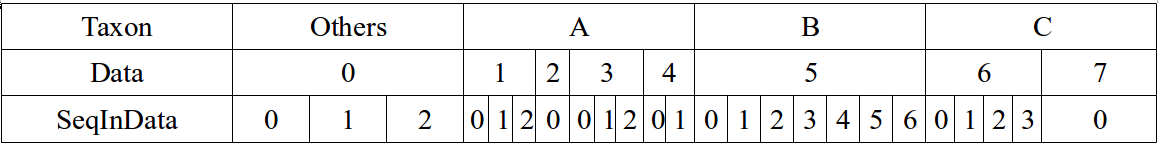
\includegraphics[scale=0.34]{./../img/map.png}
\caption{\label{map} Map dans le cas de la structure donnée en figure \ref{struct}, avec comme racine taxon\_\_alpha}
\end{center}
\end{figure}
~\\

Il est possible à présent,  à partir d'une ligne, de savoir à quelle séquence de quel jeu de données et surtout à quel taxon correspond la ligne de fréquence. C'est un bon point pour plus tard dans le développement des outils, en particulier pour l'écriture du fichier d’apprentissage puisque le taxid est la donnée à apprendre et donc à prédire. 
\\


Lors du test du programme sur une autre machine, il y a eu des erreurs avec les tests 15 à 18. Ceci est dû fait que lors de la lecture des sous dossier par l'appel système readdir, c++ ne garantie pas d'ordre. Un trie est alors effectue sur les chemins. C'est une étape qui permet au bon déroulement des tests 15 à 18 sur n'importe quel machine. Cependant il est possible de se passer du trie, dans ce cas le tableau de fréquence sera dans un ordre différent mais avec les cartes cela ne pose pas de soucis. 
